\chapter{Model evaluation} \label{ch:model_evaluation}

\section{Metrics for evaluating model performance} \label{sec:model_metrics}

\section{Model performance} \label{sec:model_performance}

Model hyperparameters were tuned for each classifier using $k$-fold cross validation, as was described in section~\ref{sec:tuning_hyperparameters}.
After the tuning, performance of the following models have been compared:

\begin{itemize}
    \item Perceptron learning algorithm, learning rate $\eta=0.5$, maximum iterations=5, features transformed with quantile transformation (uniform PDF)

    model code: ppn\_qu\_eta0.5\_maxiter5

    \item Logistic regression, L2 regularization, regularization parameter $C=0.1$, maximum iterations=100, features transformed with quantile transformation (uniform PDF)

    model code: lr\_l2\_c0.1\_maxiter\_100

    \item Logistic regression, L1 regularization, regularization parameter $C=0.1$, maximum iterations=100, features transformed with quantile transformation (uniform PDF)

    model code: lr\_l1\_c0.1\_maxiter\_100

    \item Linear Discriminant Analysis, features transformed with quantile transformation (uniform PDF)

    model code: lda

    \item Quadratic Discriminant Analysis, features transformed with quantile transformation (uniform PDF)

    model code: qda

    \item Linear Support Vector Classification, L2 regularization, regularization parameter $C=0.1$, maximum iterations=100, features transformed with quantile transformation (uniform PDF)

    model code: lsvc\_l2\_c0.1\_maxiter\_100

    \item Linear Support Vector Classification, L1 regularization, regularization parameter $C=0.1$, maximum iterations=100, features transformed with quantile transformation (uniform PDF)

    model code: lsvc\_l1\_c0.1\_maxiter\_100

    \item Gaussian Naive Bayes

    model code: nb

    \item Decision Tree, Gini impurity criterion, maximum depth of the tree=25, unscaled features

    model code: tree25

    \item Random Forest, Gini impurity criterion, number of estimators=50, unscaled features

    model code: forest50

    \item K-Nearest Neighbors, Manhattan distance metric, number of neighbors=4, standardized features

    model code: knn\_p1\_k4
\end{itemize}

Four different subsets of data have been used to test the model: train, test, and two additional validation subsets.
The train and test subsets represent Teranet records from 2011 to 2014 randomly sampled into 70\% train and 30\% test subsets;
these are the primary subsets that were used for training and tuning the hyperparameters and then evaluating the performance of classifiers on unseen test data.
The two additional validation subsets are composed of Teranet records from 2010 and 2015.
Since the land use information from Department of Geography was collected in 2012 and 2013, it can be less accurate for these subsets;
these subsets have not been used for model training or selection, but are presented as an additional reference for the generalization of performance of classifiers.
Figure~\ref{fig:model_performance} presents model performance on train, test, and two additional validation subsets.

\begin{figure}[hbt!]
    \centering
    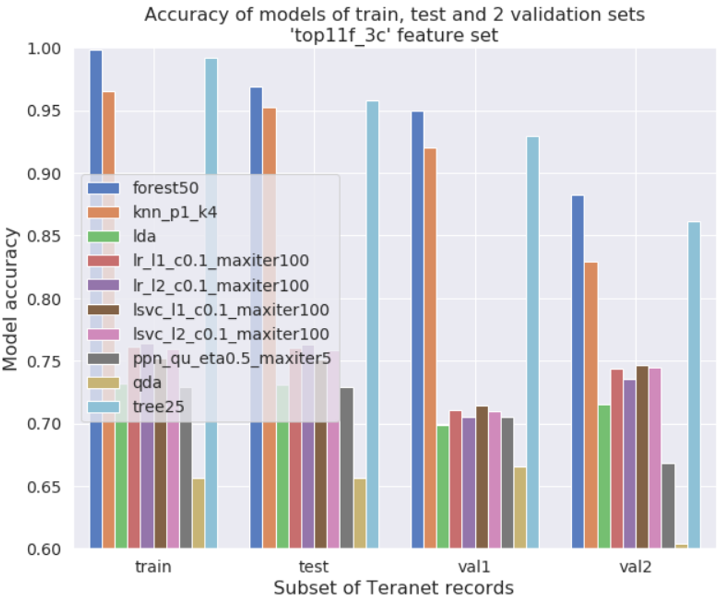
\includegraphics[width=0.6\linewidth,trim=0 0 0 0,clip]{model_performance.png}
    \caption{Model performance (accuracy) on train, test, and two additional validation subsets.
    Additional validation subsets are composed of Teranet records from 2010 and 2015;
    since land use information (target variable) can be less accurate for records in these subsets, they have been used as an additional reference for evaluating the generalization of the classifier performance.}
    \label{fig:model_performance}
\end{figure}

Different feature scaling techniques have a strong effect on model fit times and predictive performance of linear models, as can be seen on figure~\ref{fig:fit_times_linear}.

\begin{figure}[hbt!]
    \centering
    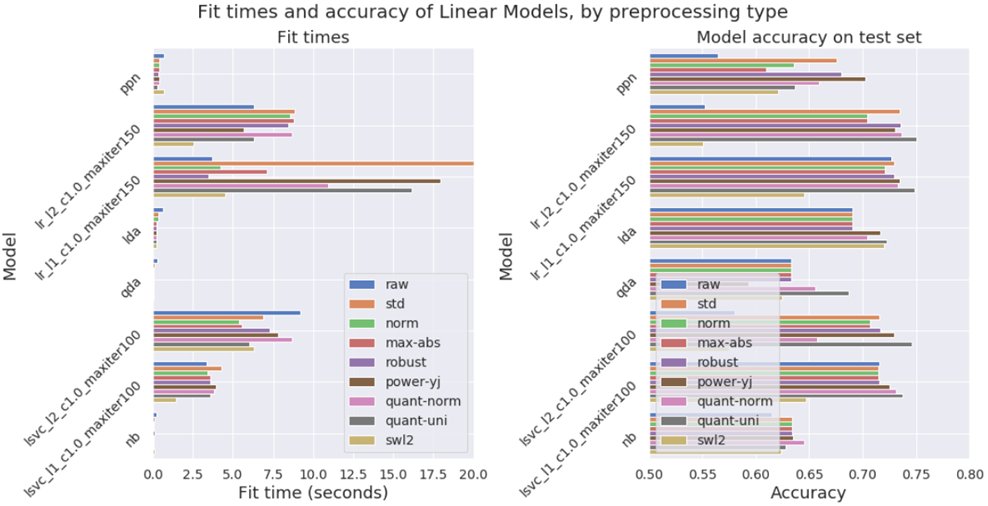
\includegraphics[width=0.98\linewidth,trim=0 0 0 0,clip]{fit_times_linear.png}
    \caption{Fit times and accuracy of linear models, by feature scaling technique.
    Different scaling techniques have a strong effect on the performance of linear models.}
    \label{fig:fit_times_linear}
\end{figure}

Similar to linear models, distance-based algorithms, such as K-Nearest Neighbors, also are strongly affected by feature scaling.
In contrast, tree-based models, such as Decision Tree and Random Forest, are scale-invariant, and thus have stable performance with most feature scaling techniques.
Figure~\ref{fig:fit_times_trees_neighbors} presents fit times for Decision Tree, Random Forest, and K-Nearest Neighbors with Manhattan and Euclidean distance metrics.


\begin{figure}[ht]
    \centering
    \begin{subfigure}{\linewidth}
        \centering
        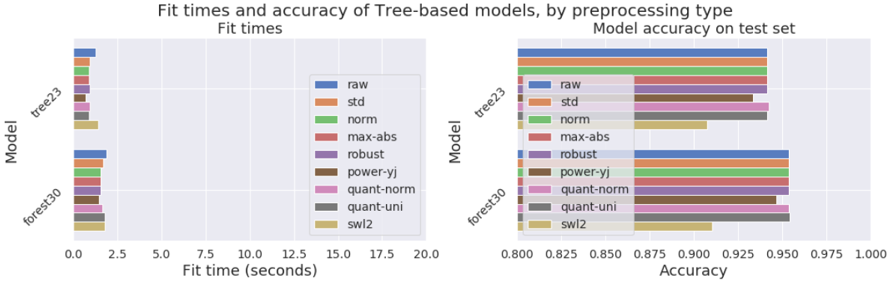
\includegraphics[width=.98\linewidth]{fit_times_trees.png}
        \label{fig:fit_times_trees}
        \caption{Tree-based models: Decision Tree and Random Forest}
    \end{subfigure}

    \begin{subfigure}{\linewidth}
        \centering
        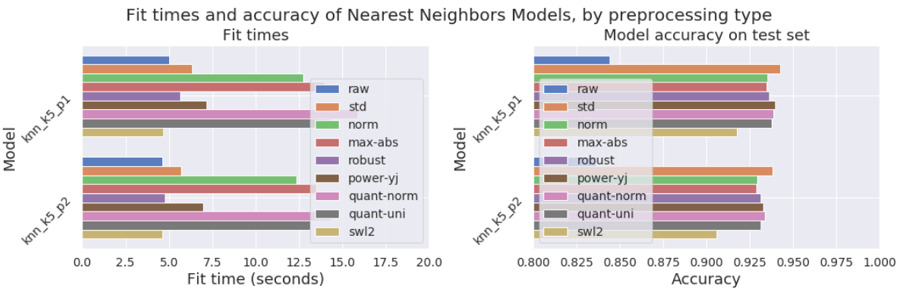
\includegraphics[width=.98\linewidth]{fit_times_neighbors.png}
        \label{fig:fit_times_neighbors}
        \caption{K-Nearest Neighbors: Manhattan and Euclidean distance}
    \end{subfigure}
    \caption{Fit times and accuracy for tree-based models and K-Nearest Neighbors, by feature scaling technique.
    Distance-based algorithms, such as K-Nearest Neighbors are affected by feature scaling, while tree-based models are scale-invariant.}
    \label{fig:fit_times_trees_neighbors}
\end{figure}

\section{Best performing model: Random Forest} \label{sec:best_performing_model}

Random Forest as can be seen from the plots presented in section~\ref{sec:model_performance}, Random Forest with 50 estimators and Gini impurity criterion showed the best results in terms of accuracy and fit times on all subsets.
Figure~\ref{fig:classification_report_train_test} presents the classification report showing all main model performance metrics for the best performing model: Random Forest with 50 estimators using 'gini' crietrion.

\begin{figure}[hbt!]
    \centering
    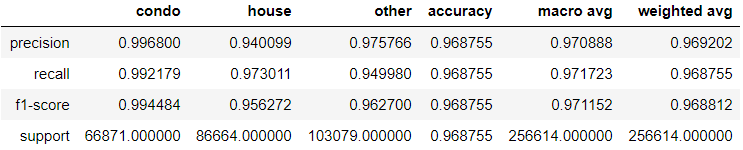
\includegraphics[width=0.98\linewidth,trim=0 0 0 0,clip]{classification_report_train_test.png}
    \caption{Best model performance on test set: classification report for Random Forest with 50 estimators using 'gini' criterion.}
    \label{fig:classification_report_train_test}
\end{figure}

Figure~\ref{fig:confusion_matrix_train_test} presents confusion matrices with and without normalization for Random Forest on the test set.

\begin{figure}[hbt!]
    \centering
    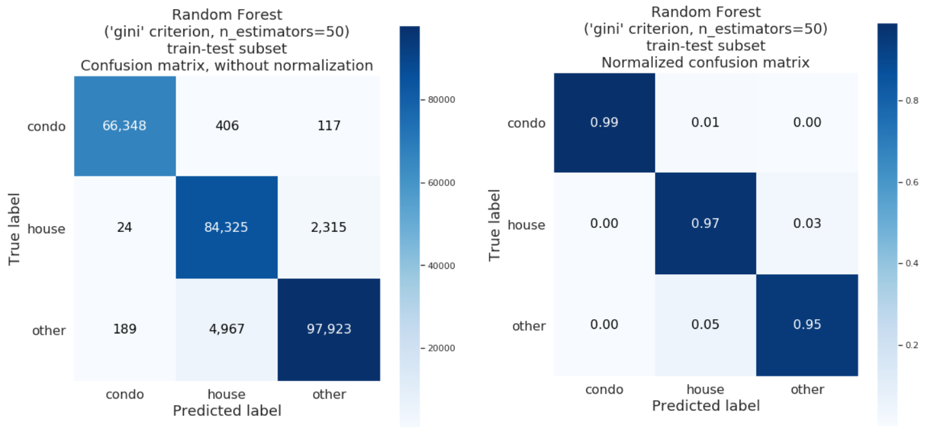
\includegraphics[width=0.98\linewidth,trim=0 0 0 0,clip]{confusion_matrix_train_test.png}
    \caption{Best model performance on test set: confusion matrices with and without normalization for Random Forest with 50 estimators using 'gini' criterion.}
    \label{fig:confusion_matrix_train_test}
\end{figure}

Figure~\ref{fig:forest_feature_importance} presents feature importance for the best performing model.

\begin{figure}[hbt!]
    \centering
    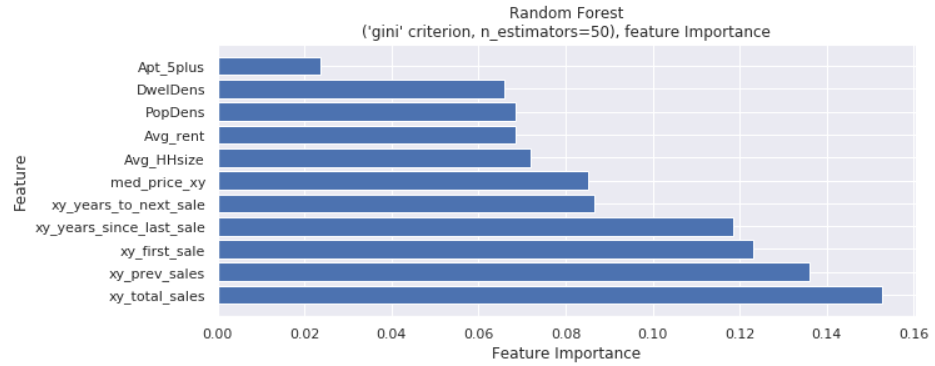
\includegraphics[width=0.98\linewidth,trim=0 0 0 0,clip]{forest_feature_importance.png}
    \caption{Random Forest with 50 estimators using 'gini' criterion: feature importance.}
    \label{fig:forest_feature_importance}
\end{figure}
